\documentclass[10pt]{article}
\usepackage[paperwidth=198mm,paperheight=59mm,margin=1mm]{geometry}
\usepackage{newtxtext,newtxmath,tikz,pgfplots}
\pgfplotsset{compat=1.18}
\definecolor{methodblue}{HTML}{216A85}
\definecolor{controlgray}{HTML}{555555}
\definecolor{accentorange}{HTML}{A64B1D}
\pagestyle{empty}
\begin{document}\noindent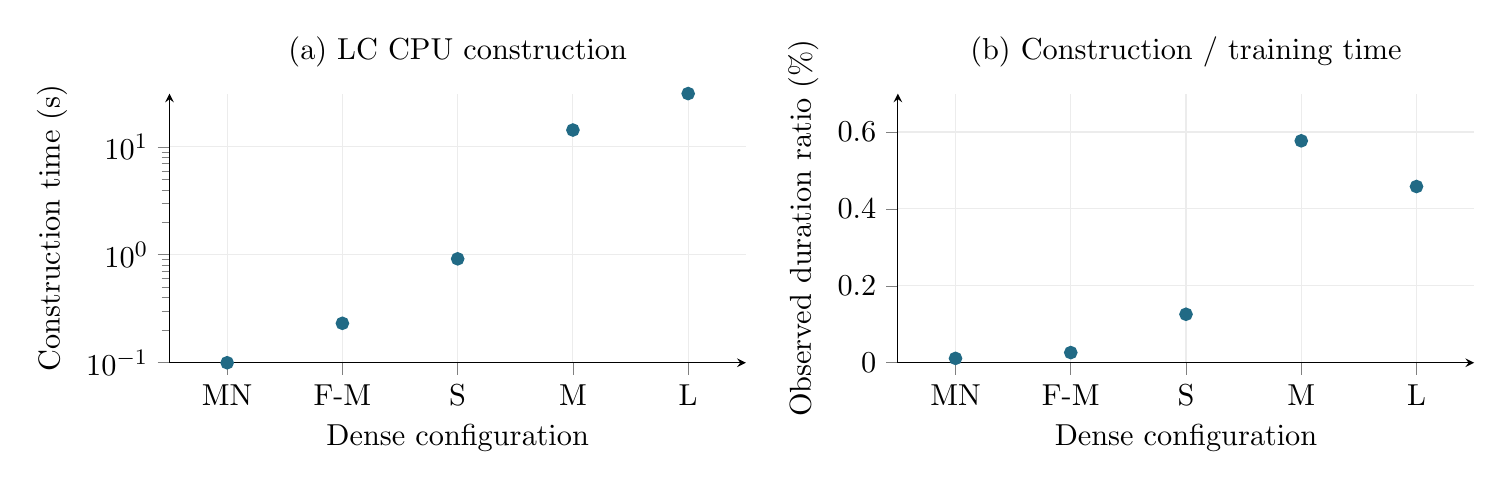
\begin{tikzpicture}
\begin{axis}[width=89mm,height=50mm,axis lines=left,tick align=outside,grid=major,grid style={gray!15},scaled ticks=false,tick label style={font=\fontsize{11}{13}\selectfont},label style={font=\fontsize{11}{13}\selectfont},title style={font=\fontsize{11}{13}\selectfont},legend style={font=\fontsize{11}{13}\selectfont,draw=none,fill=white,inner sep=1pt},title={(a) LC CPU construction},xmin=-.5,xmax=4.5,ymode=log,xtick={0,1,2,3,4},xticklabels={MN,F-M,S,M,L},xlabel={Dense configuration},ylabel={Construction time (s)}]
\addplot+[color=methodblue,mark=*,mark size=2pt,line width=0.9pt,mark options={solid,fill=methodblue,draw=methodblue},only marks] coordinates {(0,0.09968077)(1,0.23135284)(2,0.91641638)(3,14.332852)(4,31.217533)};
\end{axis}
\begin{axis}[width=89mm,height=50mm,axis lines=left,tick align=outside,grid=major,grid style={gray!15},scaled ticks=false,tick label style={font=\fontsize{11}{13}\selectfont},label style={font=\fontsize{11}{13}\selectfont},title style={font=\fontsize{11}{13}\selectfont},legend style={font=\fontsize{11}{13}\selectfont,draw=none,fill=white,inner sep=1pt},at={(9.25cm,0)},anchor=south west,title={(b) Construction / training time},xmin=-.5,xmax=4.5,ymin=0,ymax=.7,xtick={0,1,2,3,4},xticklabels={MN,F-M,S,M,L},xlabel={Dense configuration},ylabel={Observed duration ratio (\%)}]
\addplot+[color=methodblue,mark=*,mark size=2pt,line width=0.9pt,mark options={solid,fill=methodblue,draw=methodblue},only marks] coordinates {(0,0.011361538)(1,0.026421265)(2,0.12607615)(3,0.5771637)(4,0.45830137)};
\end{axis}
\end{tikzpicture}\end{document}
